\section{Anwendungen in der anorganischen Chemie}
\subsection{$^{31}$P chemische Verschiebungen in Phospor NHCs}
\ac{nhc}
\begin{figure}[ht!]
	\centering
	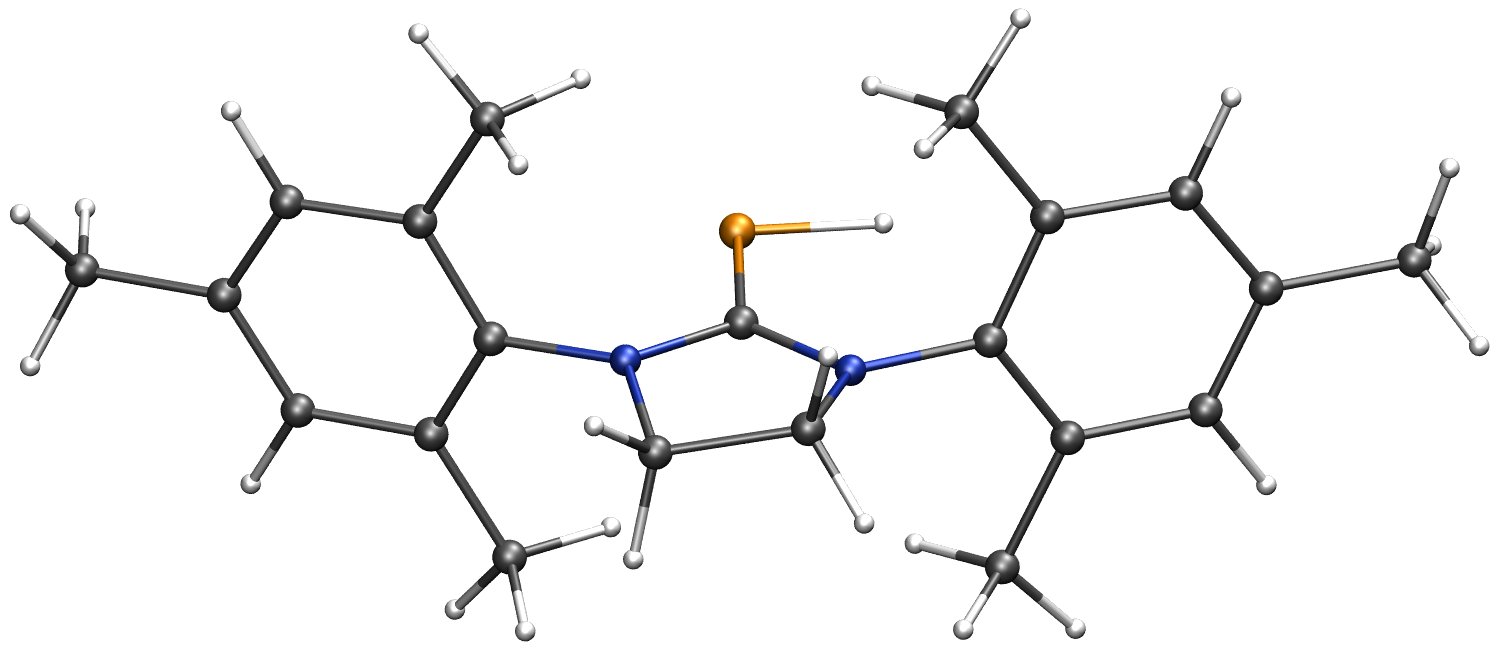
\includegraphics[width=0.6\textwidth]{1}
	\captionsetup{figurewithin = chapter}
	\captionsetup{font=small, labelfont=bf}\caption[Abbildung von SIMesPH]{Abbildung von SIMesPH, SIMes=1,3-bis(2,4,6-tri\-me\-thyl\-phe\-nyl)imi\-da\-zo\-lin-2-yli\-den (Kohlenstoff=grau, Wasserstoff=weiß, Stickstoff=blau und Phosphor=orange).}
\label{abb:cvh1}
\end{figure}

\begin{figure}[ht!]
	\centering
	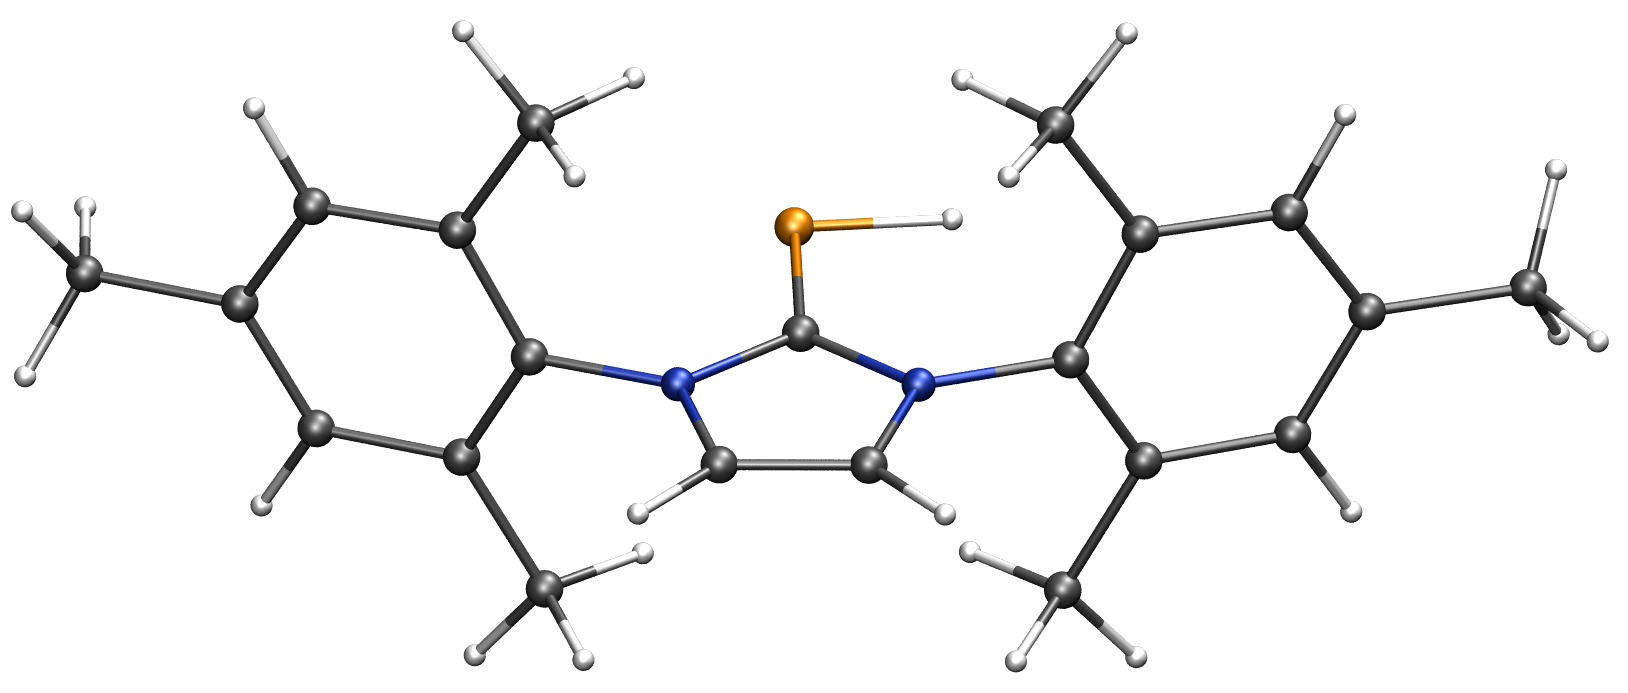
\includegraphics[width=0.6\textwidth]{2}
	\captionsetup{figurewithin = chapter}
	\captionsetup{font=small, labelfont=bf}\caption[Abbildung von IMesPH]{Abbildung von IMesPH, IMes=1,3-bis(2,4,6-tri\-me\-thyl\-phe\-nyl)imi\-da\-zol-2-yli\-den (Kohlenstoff=grau, Wasserstoff=weiß, Stickstoff=blau und Phosphor=orange).}
\label{abb:cvh2}
\end{figure}

\begin{figure}[ht!]
	\centering
	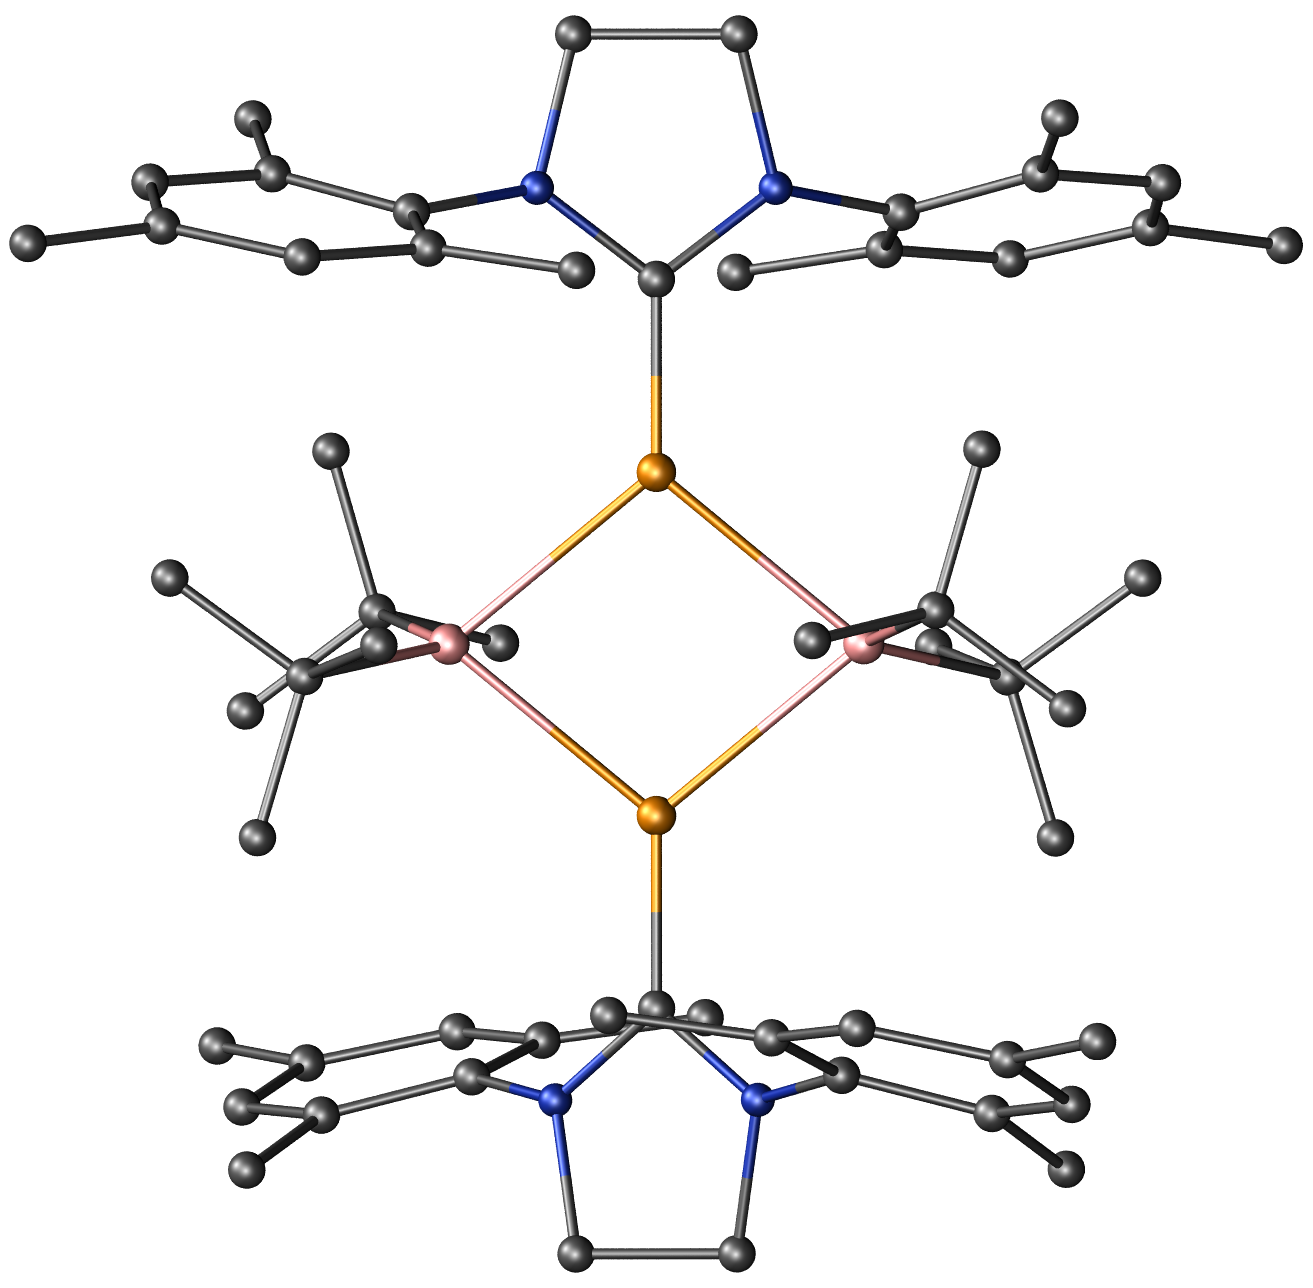
\includegraphics[width=0.6\textwidth]{3}
	\captionsetup{figurewithin = chapter}
	\captionsetup{font=small, labelfont=bf}\caption[{Abbildung von $[$SIMesPGa\textit{t}Bu$_2]_2$}]{Abbildung von $[$SIMesPGa\textit{t}Bu$_2]_2$, SIMes=1,3-bis(2,4,6-tri\-me\-thyl\-phe\-nyl)imi\-da\-zo\-lin-2-yli\-den (Kohlenstoff=grau, Stickstoff=blau, Phosphor=orange und Gallium=rosa). Die Wasserstoffatome wurden zur besseren Veranschaulichung bei der Abbildung weg gelassen.}
\label{abb:cvh3}
\end{figure}

\begin{figure}[ht!]
	\centering
	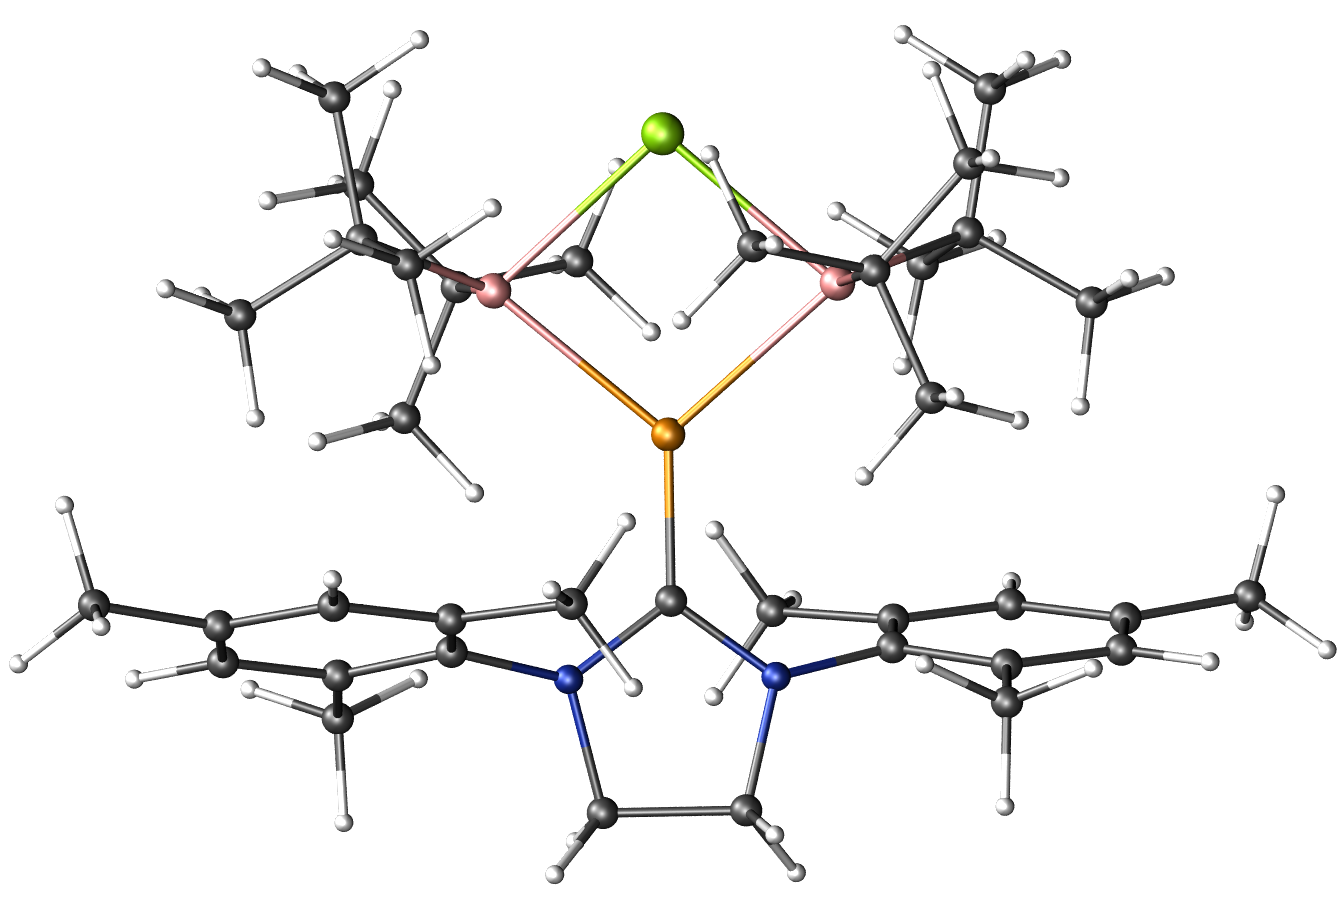
\includegraphics[width=0.6\textwidth]{4}
	\captionsetup{figurewithin = chapter}
	\captionsetup{font=small, labelfont=bf}\caption[Abbildung von SIMesP(Ga\textit{t}Bu$_2$)$_2$Cl]{Abbildung von SIMesP(Ga\textit{t}Bu$_2$)$_2$Cl, SIMes=1,3-bis(2,4,6-tri\-me\-thyl\-phe\-nyl)imi\-da\-zo\-lin-2-yli\-den (Kohlenstoff=grau, Wasserstoff=weiß, Stickstoff=blau, Phosphor=orange, Gallium=rosa und Chlor=grün).}
\label{abb:cvh4}
\end{figure}

\begin{figure}[ht!]
	\centering
	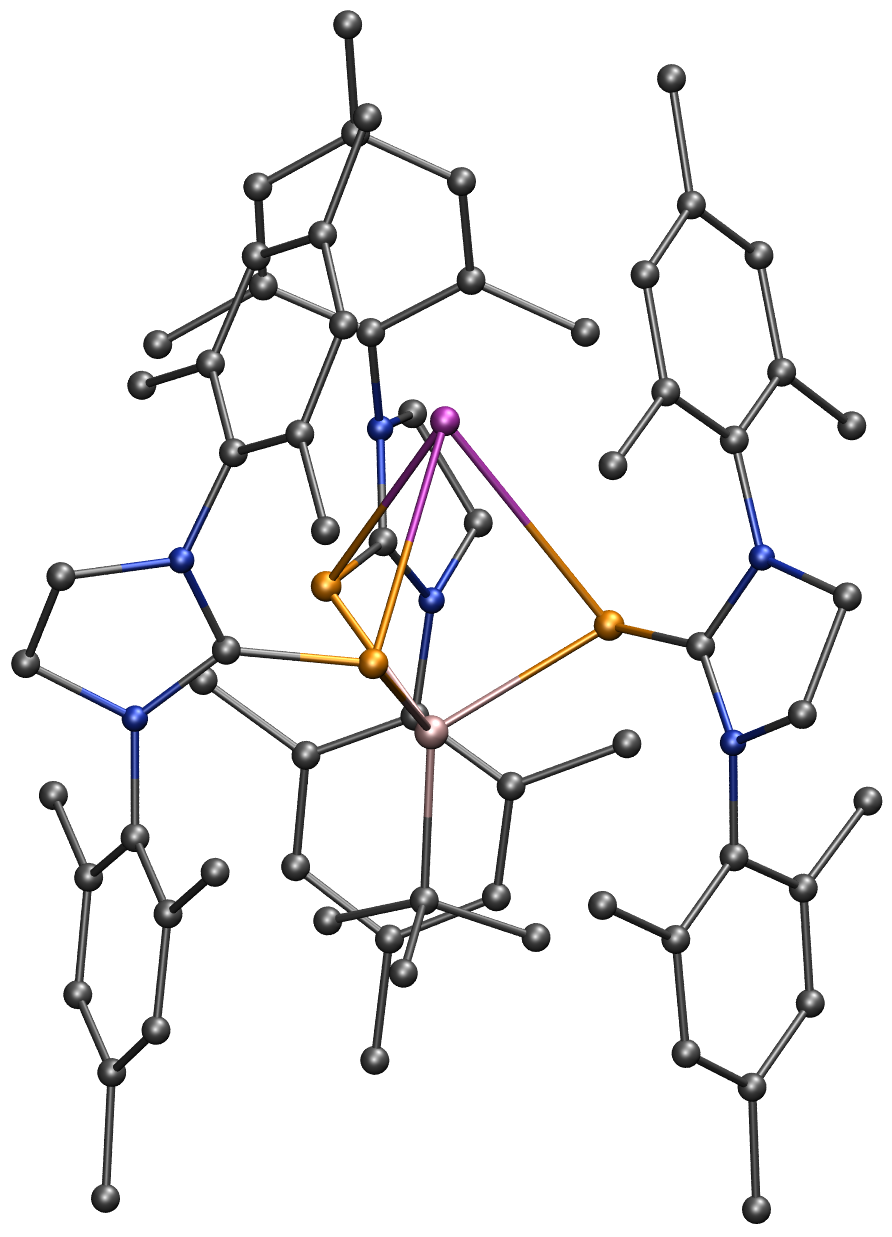
\includegraphics[width=0.5\textwidth]{5}
	\captionsetup{figurewithin = chapter}
	\captionsetup{font=small, labelfont=bf}\caption[Abbildung von K(SIMesP)$_3$Al\textit{t}Bu]{Abbildung von K(SIMesP)$_3$Al\textit{t}Bu, SIMes=1,3-bis(2,4,6-tri\-me\-thyl\-phe\-nyl)imi\-da\-zo\-lin-2-yli\-den (Kohlenstoff=grau, Stickstoff=blau, Phosphor=orange, Kalium=lila und Aluminium=hellrosa). Die Wasserstoffatome wurden zur besseren Veranschaulichung bei der Abbildung weg gelassen.}
\label{abb:cvh5}
\end{figure}

\begin{figure}[ht!]
	\centering
	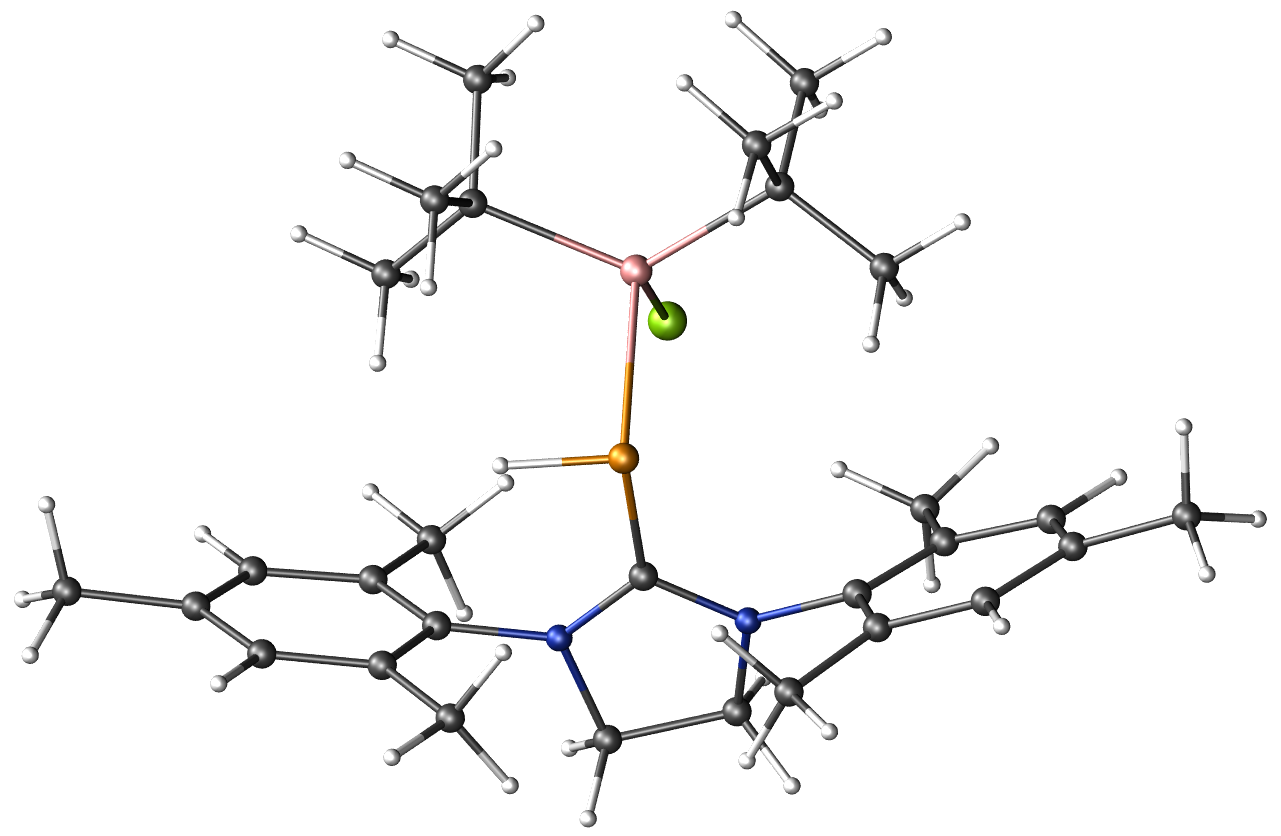
\includegraphics[width=0.6\textwidth]{6}
	\captionsetup{figurewithin = chapter}
	\captionsetup{font=small, labelfont=bf}\caption[Abbildung von SIMesPH\textit{t}Bu$_2$GaCl]{Abbildung von SIMesPH\textit{t}Bu$_2$GaCl, SIMes=1,3-bis(2,4,6-tri\-me\-thyl\-phe\-nyl)imi\-da\-zo\-lin-2-yli\-den (Kohlenstoff=grau, Wasserstoff=weiß, Stickstoff=blau, Phosphor=orange, Gallium=rosa und Chlor=grün).}
\label{abb:cvh6}
\end{figure}

\begin{figure}[ht!]
	\centering
	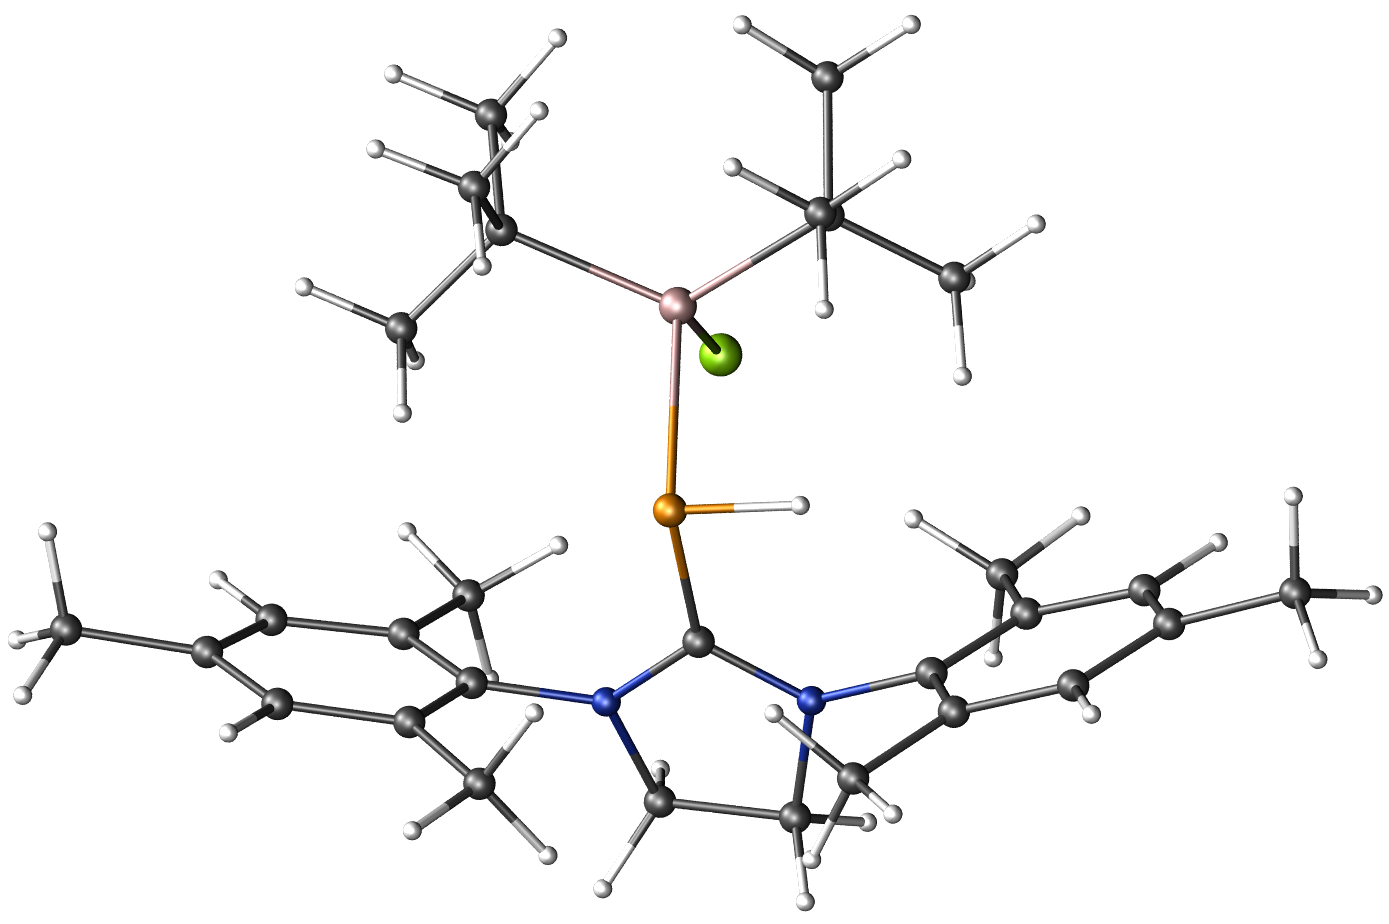
\includegraphics[width=0.6\textwidth]{7}
	\captionsetup{figurewithin = chapter}
	\captionsetup{font=small, labelfont=bf}\caption[Abbildung von SIMesPH\textit{t}Bu$_2$AlCl]{Abbildung von SIMesPH\textit{t}Bu$_2$AlCl, SIMes=1,3-bis(2,4,6-tri\-me\-thyl\-phe\-nyl)imi\-da\-zo\-lin-2-yli\-den (Kohlenstoff=grau, Wasserstoff=weiß, Stickstoff=blau, Phosphor=orange, Aluminium=hellrosa und Chlor=grün).}
\label{abb:cvh7}
\end{figure}

\begin{table}[ht!]\label{tab:cvhtab1}
\captionsetup{tablewithin = chapter}
\captionsetup{font=small, labelfont=bf}
\captionabove[Vergleich spektroskopischer und struktureller Daten für Phosphor \acp{nhc}]{Vergleich spektroskopischer und struktureller Daten für SIMesPH, IMesPH, $[$SIMesPGa\textit{t}Bu$_2]_2$, SIMesP(Ga\textit{t}Bu$_2$)$_2$Cl, K(SIMesP)$_3$Al\textit{t}Bu, SIMesPH\textit{t}Bu$_2$GaCl und SIMesPH\textit{t}Bu$_2$AlCl. }
\resizebox{\textwidth}{!}{%
\begin{tabular}{ccccccccc}
\hline \hline
Verbindung & \multicolumn{3}{c}{$^{31}$P / ppm} & \multicolumn{3}{c}{$^{13}$C (Carbenkohlenstoff) / ppm} & \multicolumn{2}{c}{P-C Abstand/ pm}\\
 & gemessen & \multicolumn{2}{c}{berechnet} & gemessen & \multicolumn{2}{c}{berechnet} &Röntgenstruktur & berechnet\\
 & & sim. $\delta ^{31}$P & $\sigma ^{31}$P & & sim. $\delta ^{13}$C & $\sigma ^{13}$C & & \\
 \hline
 SIMesPH & -127.2 & -157 & 433 & 191.0 & 192 & -3 & 174.6(2) & 175.3\\
 IMesPH & -147.3 & -178 & 454 & 180.0 & 178 & 11 & 174.7(2) & 176.1\\
 $[$SIMesPGa\textit{t}Bu$_2]_2$ & -113.2 & -57 & 333 & & 182 & 7 & 174.4(2) & 175.6\\
 SIMesP(Ga\textit{t}Bu$_2$)$_2$Cl & -122.6 & -104 & 380 & 183.3 & 181 & 8 & 175.4(1) & 175.3\\
 K(SIMesP)$_3$Al\textit{t}Bu & -61.2 & -54 & 330 & & 185 & 4 & 175.3(2) & 175.8\\
 SIMesPH\textit{t}Bu$_2$GaCl & -148.8 & -163 & 439 & 188.5 & 191 & -2 & 179.8(2) & 179.4\\
 SIMesPH\textit{t}Bu$_2$AlCl & -151.0 & -157 & 433 & 187.9 & 190 & -1 & 180.1(2) & 179.5
\end{tabular}}
\end{table}

\begin{table}[ht!]\label{tab:cvhtab2}
\captionsetup{tablewithin = chapter}
\captionsetup{font=small, labelfont=bf}
\captionabove[$^{31}$P Verschiebungen/Abschirmungen für Phosphor \acp{nhc} mit unterschiedlichen Funktionalen]{$^{31}$P Verschiebungen/Abschirmungen für SIMesPH, IMesPH, $[$SIMesPGa\textit{t}Bu$_2]_2$, SIMesP(Ga\textit{t}Bu$_2$)$_2$Cl, K(SIMesP)$_3$Al\textit{t}Bu, SIMesPH\textit{t}Bu$_2$GaCl und SIMesPH\textit{t}Bu$_2$AlCl mit unterschiedlichen Funktionalen. Die Spalte PBE, opt enthält die berechneten Werte für optimierte Strukturparameter. Alle Werte in den darauf folgenden Spalten wurden auf Grundlage der experimentellen Strukturparametern berechnet. Alle Werte sind in ppm angegeben.}
\resizebox{\textwidth}{!}{%
\begin{tabular}{cccccccccccccc}
\hline \hline
Verbindung &gemessen &\multicolumn{2}{c}{PBE, opt} &\multicolumn{2}{c}{PBE} &\multicolumn{2}{c}{BP} &\multicolumn{2}{c}{B3-LYP} &\multicolumn{2}{c}{PBE0} &\multicolumn{2}{c}{HF}\\
& & $\delta ^{31}$P & $\sigma ^{31}$P & $\delta ^{31}$P & $\sigma ^{31}$P & $\delta ^{31}$P & $\sigma ^{31}$P & $\delta ^{31}$P & $\sigma ^{31}$P & $\delta ^{31}$P & $\sigma ^{31}$P & $\delta ^{31}$P & $\sigma ^{31}$P\\
\hline
SIMesPH &-127,2 &-157 &433 &-164 &455 &-165 &450 &-163 &443 &-155 &465 &-140 &491\\
IMesPH &-147,3 &-178 &454 &-137 &428 &-138 &423 &-136 &416 &-133 &443 &-121 &472\\
$[$SIMesPGa\textit{t}Bu$_2]_2$ &-113,2 &-57  &333 &-59  &350 &-58  &343 &-61  &341 &-68  &378 &-94  &445\\
SIMesP(Ga\textit{t}Bu$_2$)$_2$Cl &-122,6 &-104 &380 &-109 &400 &-107 &392 &-111 &391 &-117 &427 &-137 &488\\
K(SIMesP)$_3$Al\textit{t}Bu &-61,2  &-54  &330 &-77  &368 &-77  &362 &-79  &359 &-83  &393 &-99  &450\\
SIMesPH\textit{t}Bu$_2$GaCl &-148,8 &-163 &439 &-162 &453 &-162 &447 &-162 &442 &-160 &470 &-144 &495\\
SIMesPH\textit{t}Bu$_2$AlCl &-151   &-157 &433 &-163 &454 &-164 &449 &-161 &441 &-158 &468 &-137 &488\\
\end{tabular}}
\end{table}
\newpage
\subsection{$[$Hg$_8$Te$_8$(Te$_2$)$_4$]$^{8-}$: Ein anorganisches Porphyrin?}
Die Implementierung des \ac{cosmo} und der \acp{ecp} in das \texttt{mpshift} Modul lieferte die notwendigen Voraussetzungen, um einen tieferen Einblick über magnetische Eigenschaften in anionischen Verbindungen, welche schwere Elemente beinhalten, zu erhalten. Ein Beispiel dafür ist das in der Gruppe von Stephanie Dehnen synthetisierte $[$Hg$_8$Te$_8$(Te$_2$)$_4$]$^{8-}$\supercite{dehnenhg4te8}, welches in Abbildung \ref{abb:hg8te16} gezeigt ist. Die Seitenansicht (Abbildung \ref{abb:hg8te16} rechts) zeigt das Molekül mit TPSSh\supercite{tao2003climbing}/def2-TZVP\supercite{weigend2005balanced} optimierten Strukturparametern. Dabei ist zu erkennen, dass das Anion nicht vollständig planar ist und damit auch leicht von der idealen $D_{4\textrm{h}}$ symmetrischen Struktur abweicht. 
\begin{figure}[ht!]
	\centering
	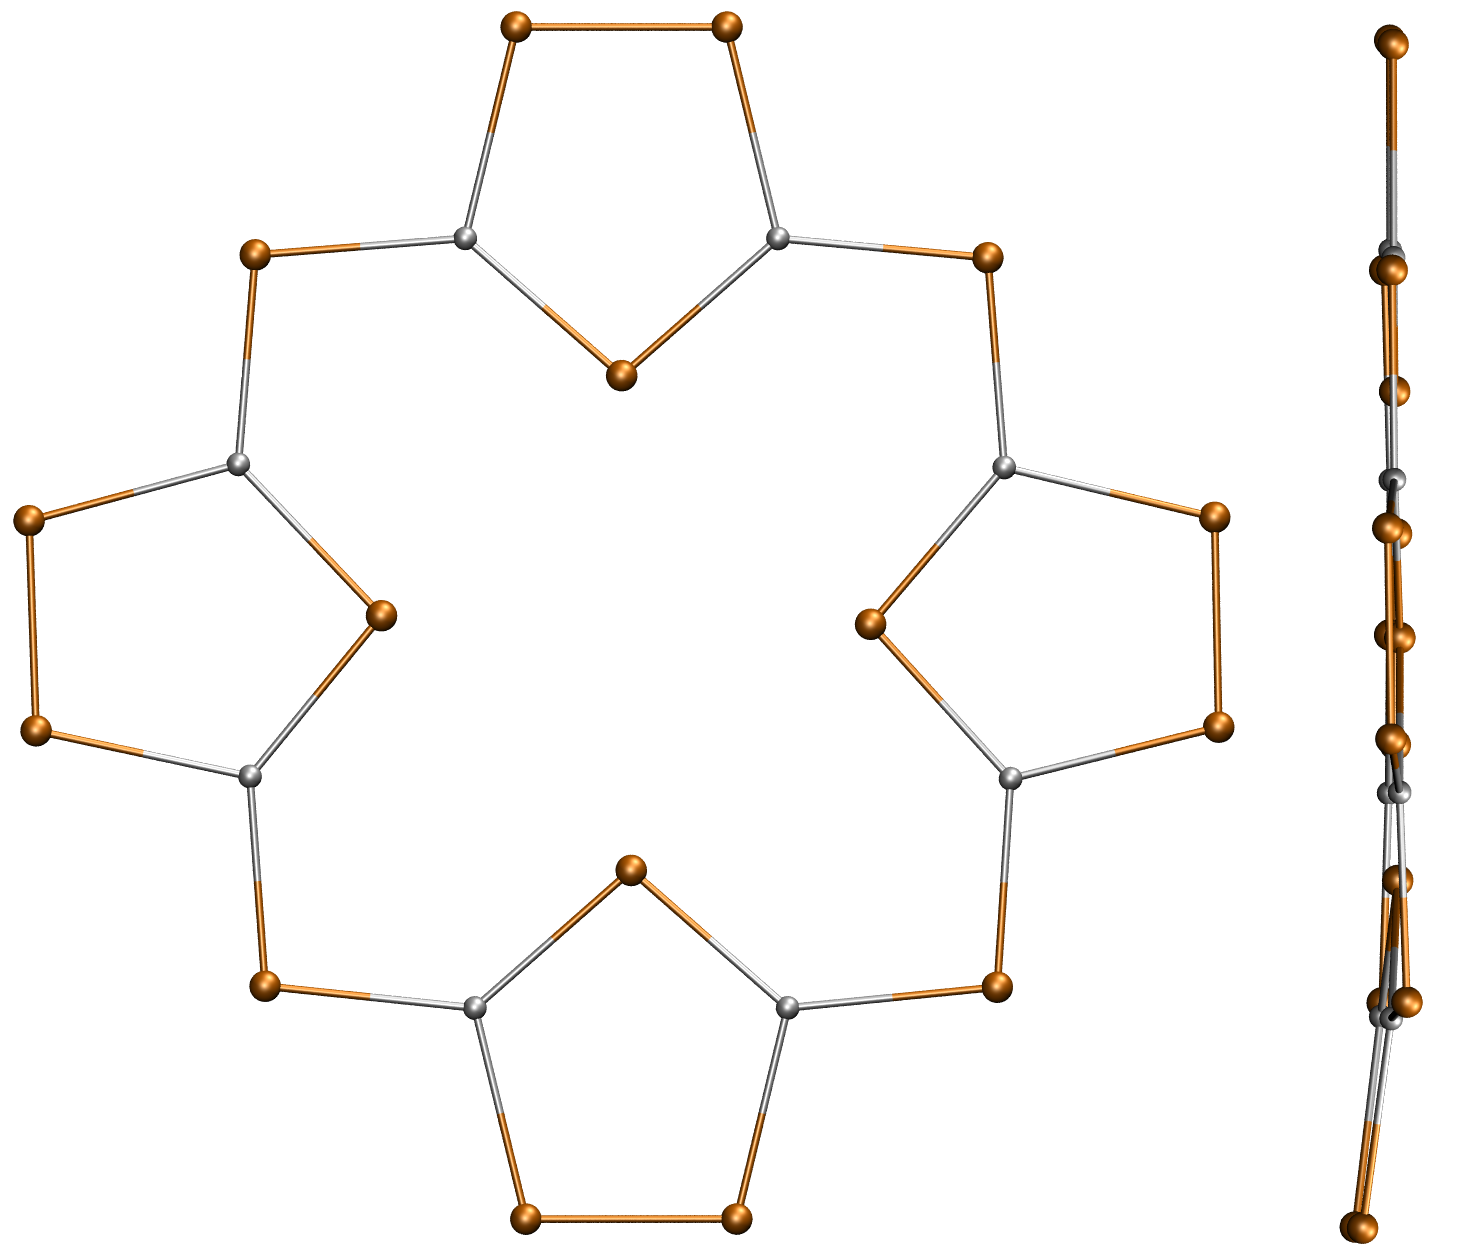
\includegraphics[width=0.6\textwidth]{hg8te16}
	\captionsetup{figurewithin = chapter}
	\captionsetup{font=small, labelfont=bf}\caption[{Abbildung von $[$Hg$_8$Te$_{16}]^{8-}$}]{{Abbildung von $[$Hg$_8$Te$_{16}]^{8-}$}(Quecksilber=silber, Tellur=orangebraun). Draufsicht links und Seitenansicht rechts.}
\label{abb:hg8te16}
\end{figure}

Zusätzlich wurde ebenfalls das bereits bekannte B$_8$S$_{16}$\supercite{krebs1980b8s16} (Abbildung \ref{abb:b8s16}) untersucht. Hier ist die Abweichung des Moleküls mit optimierten Strukturparametern von der planaren Struktur noch deutlich größer, wie die Seitenansicht deutlich zeigt. Die $D_{4\textrm{h}}$ symmetrische Struktur weißt eine schwache imaginäre Mode von etwa -10 Wellenzahlen auf welche genau der Gerüstschwingung entspricht, welche das Durchschwingen des Moleküls beschreibt. Ebenfalls bekannt ist das schwerer Homolog B$_8$Se$_{16}$.
\begin{figure}[ht!]
	\centering
	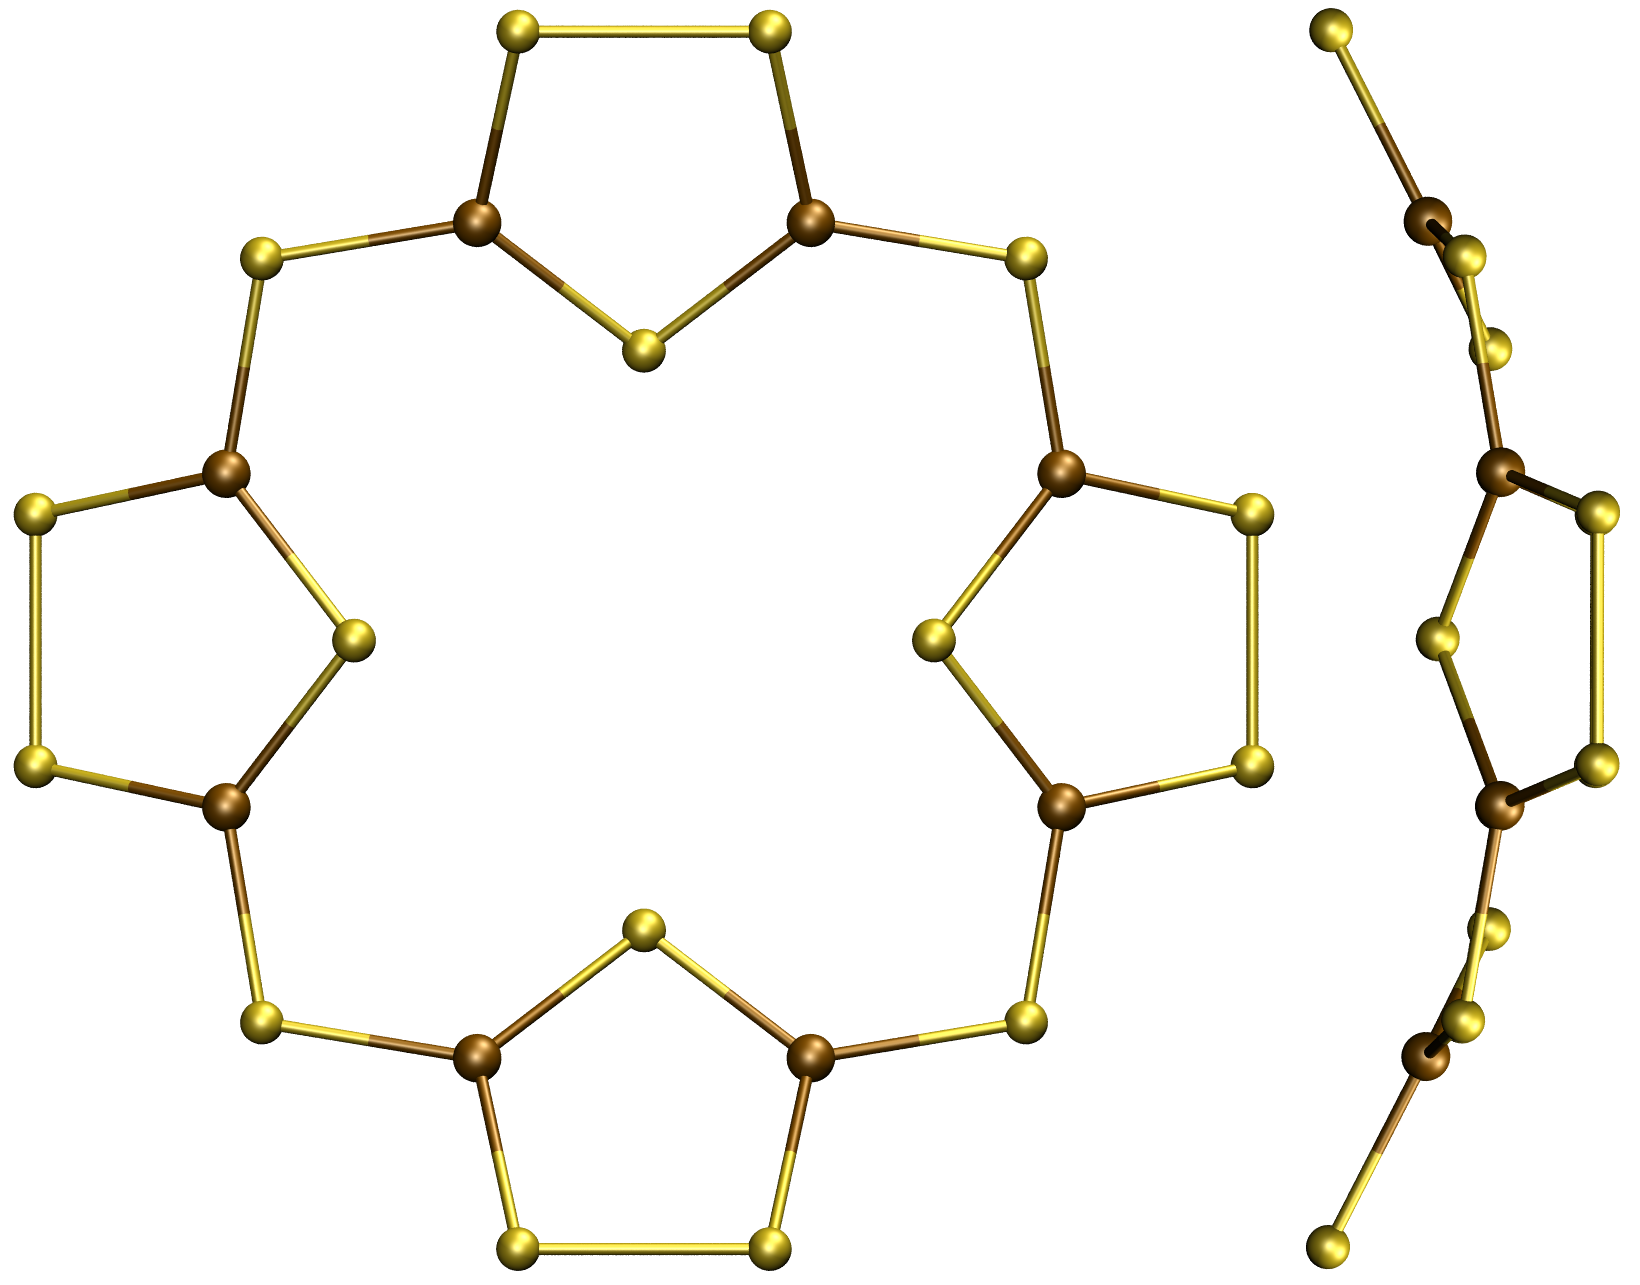
\includegraphics[width=0.6\textwidth]{b8s16}
	\captionsetup{figurewithin = chapter}
	\captionsetup{font=small, labelfont=bf}\caption[Abbildung von B$_8$S$_{16}$]{Abbildung von B$_8$S$_{16}$(Bohr=braun, Schwefel=gelb). Draufsicht links und Seitenansicht rechts.}
\label{abb:b8s16}
\end{figure}

Aufgrund ihrer strukturellen Ähnlichkeit mit dem organischen Porphyrin lag es nahe, den aromatischen Charakter der Verbindungen zu untersuchen. Als Maß für die Aromatizität einer Verbindung kann der durch einen definierten Ring fließende Elektronenstrom angesehen werden. Je diatropischer der Gesamtstrom (d.h. der Strom fließt im Uhrzeigersinn), desto aromatischer ist die Verbindung. Ein stark paratropischer Strom (Strom entgegen des Uhrzeigersinns) deutet dabei auf eine antiaromatische Verbindung hin. Sind die diatropischen und paratropischen Beiträge in etwa von der selben Größe, dann verschwindet der Gesamtstrom - die Verbindung ist nichtaromatisch. Bei der Berechnung der Ringströme mit \ac{gimic} wird dabei so vorgegangen, dass der Strom der durch eine senkrecht zur Bindungsachse stehenden Ebene fließt integriert wird. In beiden oben erwähnten Beispielen kann weiterhin zwischen einem lokalen Ringstrom in den vier Fünfringen und einem globalen Ringstrom um das gesamte Molekül unterschieden werden. Bei den Berechnungen hat sich herausgestellt, dass alle drei Verbindungen, $[$Hg$_8$Te$_{16}]^{8-}$, B$_8$S$_{16}$ und B$_8$Se$_{16}$ einen schwachen lokalen Ringstrom in den pyrrolartigen fünfgliedrigen Ringen aufweisen. Diese betragen \unit[5.8]{nA/T} in $[$Hg$_8$Te$_{16}]^{8-}$ \unit[3.25]{nA/T} in B$_8$S$_{16}$ und \unit[3.28]{nA/T} in B$_8$Se$_{16}$. Im Vergleich dazu beträgt der Ringstrom in einem Benzolmolekül etwa \unit[12]{nA/T}\supercite{fliegl2012aromatic}. Die globalen Ringströme in den drei Verbindungen sind mit \unit[0.24]{nA/T}, \unit[0.81]{nA/T} und \unit[0.79]{nA/T} verschwindend gering. Im Vergleich dazu liegt der globale Ringstrom des organischen Porphyrins bei etwa \unit[27]{nA/T}. Dieser spaltet sich in den Fünfgliedrigen Ringen in einen äußeren und inneren Pfad auf, welche bei jeweils einen Ringstrom von etwa \unit[13]{nA/T} aufweisen. Der lokale Ringstrom in den fünfgliedrigen Ringen ist schwächer als \unit[1]{nA/T}.\supercite{fliegl2012aromatic} In sogenannten \ac{lic} Plots lassen sich die Ringströme in einer gewählten Ebene visualisieren. Dies wurde für das organische Porphyrin und die drei Verbindungen $[$Hg$_8$Te$_{16}]^{8-}$, B$_8$S$_{16}$ und B$_8$Se$_{16}$ gemacht und die entsprechenden Plots sind in den Abbildungen \ref{abb:porphlic} bis \ref{abb:b8se16hlic} zu sehen. Beim Porphyrin ist eindeutig der globale Ringstrom zu erkenne, welcher sich in den fünfgliedrigen Ringen in zwei Pfade aufspaltet. im Vergleich dazu weisen die anderen Verbindungen lediglich lokale Ströme in den fünfgliedrigen Ringen auf.

\begin{figure}[ht!]
	\centering
	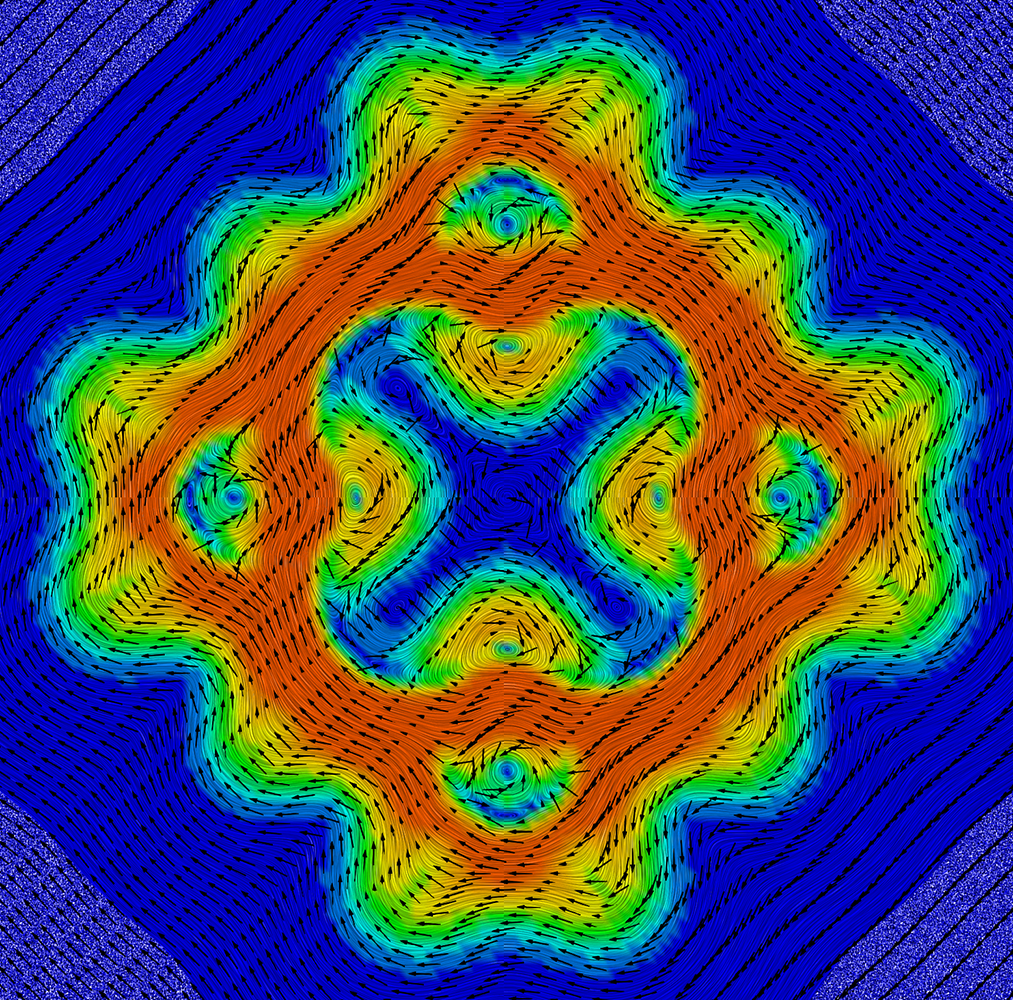
\includegraphics[width=0.6\textwidth]{porph_1bohr}
	\captionsetup{figurewithin = chapter}
	\captionsetup{font=small, labelfont=bf}\caption[Ringströme in Porphyrin]{Ringströme in Porphyrin \unit[1]{bohr} oberhalb der Molekülebene, dargestellt zwischen \unit[0]{a.u.} (blau) und \unit[0.07]{a.u.}.}
\label{abb:porphlic}
\end{figure}

\begin{figure}[ht!]
	\centering
	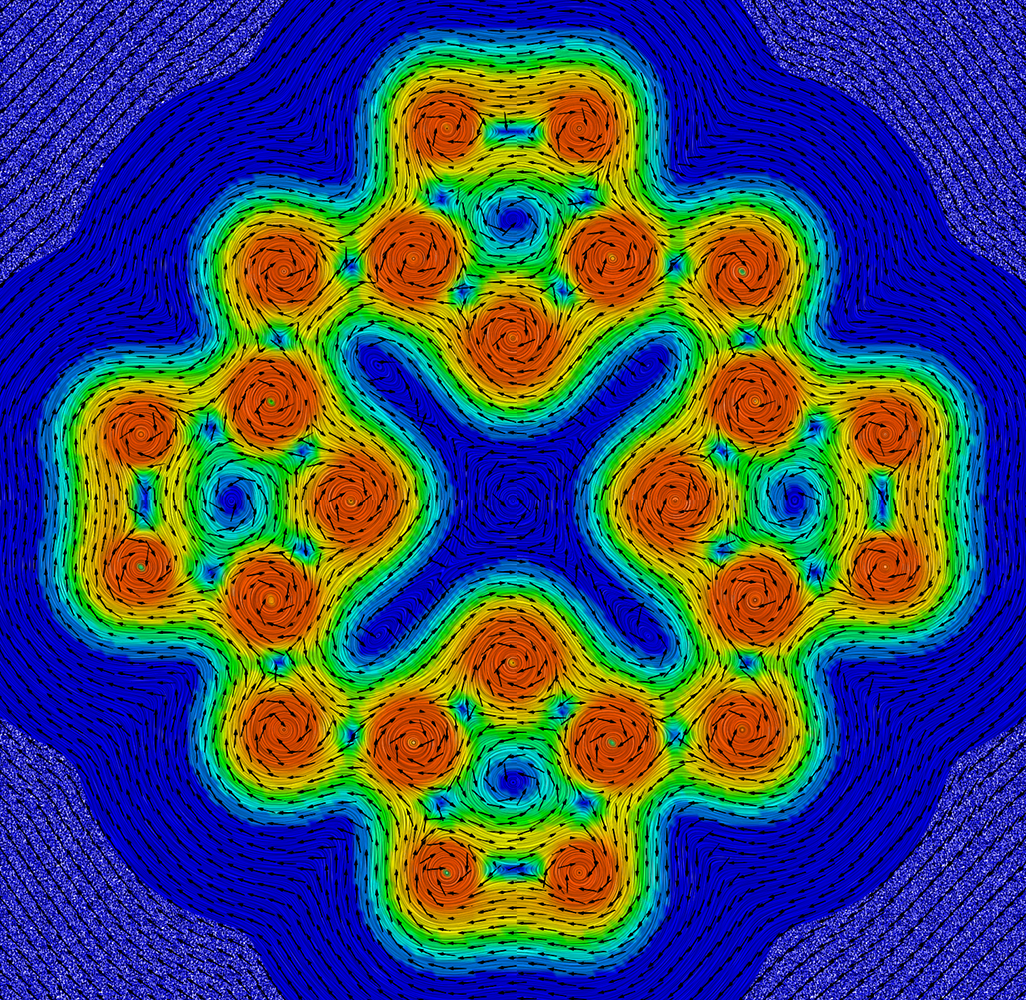
\includegraphics[width=0.6\textwidth]{hgte_1bohr}
	\captionsetup{figurewithin = chapter}
	\captionsetup{font=small, labelfont=bf}\caption[{Ringströme in $[$Hg$_8$Te$_8$(Te$_2$)$_4]^{8-}$}]{Ringströme in $[$Hg$_8$Te$_8$(Te$_2$)$_4]^{8-}$ \unit[1]{bohr} oberhalb der Molekülebene, dargestellt zwischen \unit[0]{a.u.} (blau) und \unit[0.07]{a.u.}.}
\label{abb:hgtelic}
\end{figure}

\begin{figure}[ht!]
	\centering
	\includegraphics[width=0.6\textwidth]{b8s16_1bohr}
	\captionsetup{figurewithin = chapter}
	\captionsetup{font=small, labelfont=bf}\caption[Ringströme in B$_8$S$_{16}$]{Ringströme in B$_8$S$_{16}$ \unit[1]{bohr} oberhalb der Molekülebene, dargestellt zwischen \unit[0]{a.u.} (blau) und \unit[0.07]{a.u.}.}
\label{abb:b8s16hlic}
\end{figure}

\begin{figure}[ht!]
	\centering
	\includegraphics[width=0.6\textwidth]{b8se16_1bohr}
	\captionsetup{figurewithin = chapter}
	\captionsetup{font=small, labelfont=bf}\caption[Ringströme in B$_8$Se$_{16}$]{Ringströme in B$_8$Se$_{16}$ \unit[1]{bohr} oberhalb der Molekülebene, dargestellt zwischen \unit[0]{a.u.} (blau) und \unit[0.07]{a.u.}.}
\label{abb:b8se16hlic}
\end{figure}
\newpage
\subsection{[Co\@Sn$_6$Sb$_6$]$^{3-}$}
\newpage
\section{Ringströme in großen ringförmigen Kohlenstoffnanoröhren}